\documentclass[11pt,a4paper]{article}

\usepackage[T1]{fontenc}
\usepackage[utf8]{inputenc}
\usepackage{mathpazo}
\usepackage[scaled=0.90]{helvet}
\usepackage{courier}
\usepackage{microtype}
\usepackage[margin=0.85in,headheight=15pt]{geometry}
\usepackage{amsmath,amssymb}
\usepackage{booktabs,longtable,tabularx,array}
\usepackage{enumitem}
\usepackage[table]{xcolor}
\usepackage{listings}
\usepackage{tcolorbox}
\usepackage{tikz}
\usetikzlibrary{arrows.meta,positioning,shapes.geometric,fit,backgrounds,calc}
\usepackage{fancyhdr}
\usepackage{titlesec}
\usepackage[obeyspaces,spaces]{url}
\usepackage{hyperref}
\sloppy
\emergencystretch=3em

\definecolor{arknavy}{HTML}{0F2537}
\definecolor{arkblue}{HTML}{1B4F72}
\definecolor{arkteal}{HTML}{117864}
\definecolor{arkgold}{HTML}{B7950B}
\definecolor{arkgray}{HTML}{F4F6F7}
\definecolor{arkborder}{HTML}{D0D3D4}
\definecolor{codebg}{HTML}{F8F9F9}

\hypersetup{
  colorlinks=true,
  linkcolor=arkblue,
  urlcolor=arkteal,
  citecolor=arkblue,
  pdftitle={Arkantos AI Stack Suite - Comprehensive Architectural and Engineering Reference Manual},
  pdfauthor={Kival},
  pdfsubject={Pure Native C++20/C++23 High-Performance AI, Cognitive Agent, MLOps, and Scientific Computing Stack},
  pdfkeywords={Arkantos, Sphinx, Sutra, Milda, Vach, Yantra, Darshana, Surya, Obsidian, Basalt, Bellows, Hyper Math, C++23, GPLv3}
}

\pagestyle{fancy}
\fancyhf{}
\fancyhead[L]{\footnotesize\sffamily\textbf{Arkantos AI Stack Suite} --- Architectural \& Engineering Reference Manual}
\fancyhead[R]{\footnotesize\sffamily GPLv3+ (\copyright\ 2026 Kival)}
\fancyfoot[L]{\footnotesize\sffamily Reference Workstation: \texttt{Silver} (i7-12700K 12C + 48 GiB DDR4 + RTX 3070 8 GiB)}
\fancyfoot[R]{\footnotesize\sffamily Page \thepage}
\renewcommand{\headrulewidth}{0.4pt}
\renewcommand{\footrulewidth}{0.4pt}

\titleformat{\section}
  {\Large\sffamily\bfseries\color{arknavy}}
  {\thesection.}{0.6em}{}[\titlerule]
\titleformat{\subsection}
  {\large\sffamily\bfseries\color{arkblue}}
  {\thesubsection}{0.6em}{}
\titleformat{\subsubsection}
  {\normalsize\sffamily\bfseries\color{arkteal}}
  {\thesubsubsection}{0.5em}{}

\lstset{
  basicstyle=\ttfamily\footnotesize,
  backgroundcolor=\color{codebg},
  frame=single,
  rulecolor=\color{arkborder},
  breaklines=true,
  columns=fullflexible,
  keepspaces=true,
  showstringspaces=false,
  aboveskip=6pt,
  belowskip=6pt
}

\newcolumntype{Y}{>{\raggedright\arraybackslash}X}

\begin{document}

% ============================================================================
% TITLE PAGE
% ============================================================================
\begin{titlepage}
\centering
\vspace*{1.0cm}
{\scshape\Large Pure Native C++20 / C++23 Systems Engineering Documentation\par}
\vspace{0.6cm}
\rule{\textwidth}{1.5pt}\\[0.4cm]
{\Huge\sffamily\bfseries\color{arknavy} Arkantos AI Stack Suite\par}
\vspace{0.3cm}
{\Large\sffamily\bfseries\color{arkblue} Comprehensive Architectural, Algorithmic, and Systems Engineering Reference Manual\par}
\vspace{0.2cm}
\rule{\textwidth}{1.5pt}\\[0.8cm]

\begin{tcolorbox}[colback=arkgray,colframe=arknavy,title={\sffamily\bfseries Suite Scope \& Component Coverage (11 Native Engines + Stack Integration Proof)}]
\small
\begin{itemize}[leftmargin=1.5em,itemsep=2pt]
  \item \textbf{Layer 0 (Mathematical \& Classical ML Substrate):} \texttt{Hyper Math} (\texttt{libhypermath}) \& \texttt{Bellows} (\texttt{libbellows})
  \item \textbf{Layer 1 (Deep Learning, NLP, Vision \& Visualization):} \texttt{Basalt Deep Learning} (\texttt{libbasalt}), \texttt{Obsidian / ObsidianDb} (\texttt{libobsidian}), \texttt{Surya} (\texttt{libsurya}), \& \texttt{Darshana} (\texttt{libdarshana})
  \item \textbf{Layer 2 (Cryptographic MLOps, Vector Storage \& Real-Time Voice I/O):} \texttt{Yantra} (\texttt{libyantra}) \& \texttt{Vach} (\texttt{libvach})
  \item \textbf{Layer 3 (Hybrid GPU+CPU MoE Runtime \& Agent Orchestration):} \texttt{Sutra} (\texttt{libsutra})
  \item \textbf{Layer 4 (Cognitive Engineering Agent \& Polyglot Inference):} \texttt{Sphinx} (\texttt{sphinx} / \texttt{sphinx-text}) \& \texttt{Milda} (\texttt{milda})
  \item \textbf{Layer 5 (End-to-End Hardware Composability Proof):} \texttt{Stack Test} (\texttt{stack\_integration\_test})
\end{itemize}
\end{tcolorbox}

\vspace{0.5cm}

\begin{tcolorbox}[colback=white,colframe=arkteal,title={\sffamily\bfseries Reference Hardware Profile (\texttt{Silver})}]
\small
\begin{tabularx}{\textwidth}{lY}
\textbf{Operating System:} & Debian GNU/Linux 13 (Trixie), Linux Kernel \texttt{6.12.113+deb13-amd64} \\
\textbf{Processor (CPU):} & 12th Gen Intel Core i7-12700K --- \textbf{12 Physical Cores} (\texttt{8 Golden Cove P-cores} @ 2 SMT threads \texttt{[0..15]} + \texttt{4 Gracemont E-cores} @ 1 thread \texttt{[16..19]} = 20 logical CPUs; \texttt{AVX2+FMA}, \texttt{SHA-NI}, \texttt{SSE4.2 CRC32C}) \\
\textbf{System Memory:} & 48 GiB Dual-Channel DDR4 (\texttt{\textasciitilde 40.33 GiB/s} measured page-cache read bandwidth) \\
\textbf{Accelerator (GPU):} & NVIDIA GeForce RTX 3070 (\texttt{8,192 MiB GDDR6 VRAM}, Compute Capability \texttt{sm\_86}, CUDA \texttt{12.4}) \\
\textbf{Primary Storage:} & Samsung SSD 970 EVO Plus 1 TB NVMe (\texttt{ext4}, \texttt{\textasciitilde 3.3 GB/s} sequential read)
\end{tabularx}
\end{tcolorbox}

\vfill

\begin{tcolorbox}[colback=arkgray,colframe=arkblue,title={\sffamily\bfseries Copyright \& GNU GPLv3+ Documentation License Notice}]
\footnotesize
\textbf{Copyright \copyright\ 2026 Kival.} All rights reserved under the GNU General Public License.\\[3pt]
This manual and the entire \textbf{Arkantos AI Stack Suite} (source code, headers, build scripts, verification suites, and documentation) are free software and free documentation: you can redistribute them and/or modify them under the terms of the \textbf{GNU General Public License} as published by the Free Software Foundation, either version 3 of the License, or (at your option) any later version (\texttt{GPL-3.0-or-later}), with the \textbf{Section 7 Runtime \& Hardware Compute Library Exception} (permitting linking with NVIDIA CUDA, Vulkan, OpenGL/GLES, SDL3, FreeType, HarfBuzz, ONNX Runtime, \texttt{espeak-ng}, ALSA/PipeWire, \texttt{llama.cpp}/\texttt{ggml}, and \texttt{whisper.cpp}).\\[3pt]
The Arkantos AI Stack Suite follows the \textbf{GNU Coding Standards} strictly as an engineering, formatting, and verification discipline; it is an independent project and is not affiliated with or endorsed by the Free Software Foundation.
\end{tcolorbox}

\vspace{0.3cm}
{\normalsize\sffamily \textbf{Author:} Kival \quad|\quad \textbf{Version:} 1.0.0 \quad|\quad \textbf{Date:} November 9, 2026\par}
\end{titlepage}

\tableofcontents
\newpage

% ============================================================================
% SECTION 1: EXECUTIVE SUMMARY & SYSTEM TAXONOMY
% ============================================================================
\section{Executive Summary \& System Taxonomy}

The \textbf{Arkantos AI Stack Suite} is a clean-room, vertically integrated \textbf{C++20/C++23} artificial intelligence, scientific computing, MLOps, multimodal perception, and autonomous agent stack. It replaces the fragmented Python AI ecosystem (\texttt{NumPy}, \texttt{SciPy}, \texttt{Pandas}, \texttt{Polars}, \texttt{scikit-learn}, \texttt{XGBoost}, \texttt{LightGBM}, \texttt{CatBoost}, \texttt{PyTorch}, \texttt{Hugging Face Tokenizers/Transformers}, \texttt{spaCy}, \texttt{NLTK}, \texttt{Gensim}, \texttt{OpenCV}, \texttt{Albumentations}, \texttt{Ultralytics}, \texttt{Matplotlib}, \texttt{Seaborn}, \texttt{Plotly}, \texttt{MLflow}, \texttt{Prefect}, \texttt{FAISS}, \texttt{Fairlearn}, \texttt{LangChain}, \texttt{LlamaIndex}, and \texttt{AutoGen}) with \textbf{11 native C++ libraries/engines and 1 end-to-end hardware composability verification harness}.

\subsection{Five-Layer Vertical Architecture Diagram}

\begin{center}
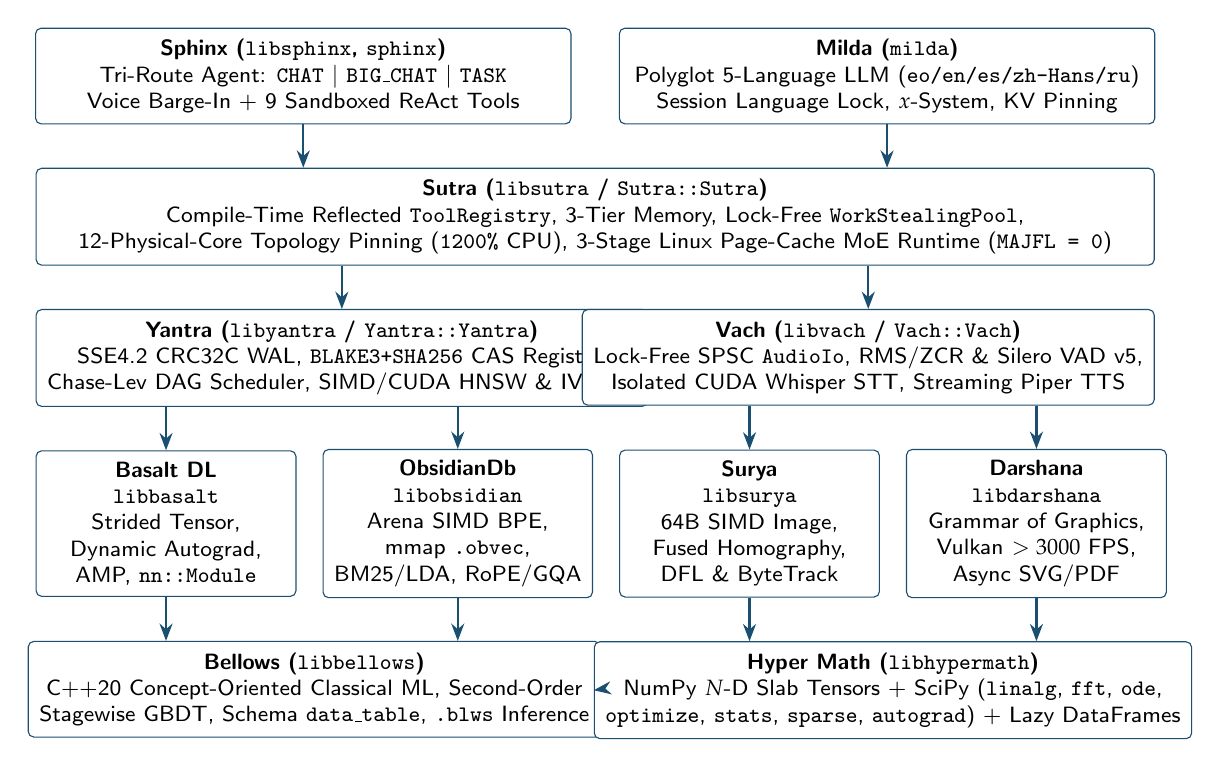
\begin{tikzpicture}[
  node distance=0.45cm and 0.5cm,
  layerbox/.style={draw=arknavy, fill=arkgray, rounded corners=3pt, inner sep=6pt},
  compbox/.style={draw=arkblue, fill=white, rounded corners=2pt, align=center, font=\sffamily\footnotesize, minimum height=1.15cm, inner sep=4pt},
  arrow/.style={-{Stealth[length=2.2mm]}, thick, color=arkblue}
]
  % Layer 4
  \node[compbox, minimum width=6.8cm] (sphinx) {\textbf{Sphinx (\texttt{libsphinx}, \texttt{sphinx})}\\Tri-Route Agent: \texttt{CHAT} $|$ \texttt{BIG\_CHAT} $|$ \texttt{TASK}\\Voice Barge-In + 9 Sandboxed ReAct Tools};
  \node[compbox, minimum width=6.8cm, right=0.6cm of sphinx] (milda) {\textbf{Milda (\texttt{milda})}\\Polyglot 5-Language LLM (\texttt{eo/en/es/zh-Hans/ru})\\Session Language Lock, $x$-System, KV Pinning};

  % Layer 3
  \node[compbox, minimum width=14.2cm, below=0.55cm of $(sphinx.south)!0.5!(milda.south)$] (sutra) {\textbf{Sutra (\texttt{libsutra} / \texttt{Sutra::Sutra})}\\Compile-Time Reflected \texttt{ToolRegistry}, 3-Tier Memory, Lock-Free \texttt{WorkStealingPool},\\12-Physical-Core Topology Pinning (\texttt{1200\%} CPU), 3-Stage Linux Page-Cache MoE Runtime (\texttt{MAJFL = 0})};

  % Layer 2
  \node[compbox, minimum width=6.8cm, below=0.55cm of sutra.south west, anchor=north west] (yantra) {\textbf{Yantra (\texttt{libyantra} / \texttt{Yantra::Yantra})}\\SSE4.2 CRC32C WAL, \texttt{BLAKE3+SHA256} CAS Registry,\\Chase-Lev DAG Scheduler, SIMD/CUDA HNSW \& IVF-PQ};
  \node[compbox, minimum width=6.8cm, below=0.55cm of sutra.south east, anchor=north east] (vach) {\textbf{Vach (\texttt{libvach} / \texttt{Vach::Vach})}\\Lock-Free SPSC \texttt{AudioIo}, RMS/ZCR \& Silero VAD v5,\\Isolated CUDA Whisper STT, Streaming Piper TTS};

  % Layer 1
  \node[compbox, minimum width=3.3cm, below=0.55cm of yantra.south west, anchor=north west] (basalt) {\textbf{Basalt DL}\\\texttt{libbasalt}\\Strided Tensor,\\Dynamic Autograd,\\AMP, \texttt{nn::Module}};
  \node[compbox, minimum width=3.3cm, right=0.33cm of basalt] (obsidian) {\textbf{ObsidianDb}\\\texttt{libobsidian}\\Arena SIMD BPE,\\mmap \texttt{.obvec},\\BM25/LDA, RoPE/GQA};
  \node[compbox, minimum width=3.3cm, right=0.33cm of obsidian] (surya) {\textbf{Surya}\\\texttt{libsurya}\\64B SIMD Image,\\Fused Homography,\\DFL \& ByteTrack};
  \node[compbox, minimum width=3.3cm, right=0.33cm of surya] (darshana) {\textbf{Darshana}\\\texttt{libdarshana}\\Grammar of Graphics,\\Vulkan $>3000$ FPS,\\Async SVG/PDF};

  % Layer 0
  \node[compbox, minimum width=6.8cm, below=0.55cm of $(basalt.south west)!0.5!(obsidian.south east)$] (bellows) {\textbf{Bellows (\texttt{libbellows})}\\C++20 Concept-Oriented Classical ML, Second-Order\\Stagewise GBDT, Schema \texttt{data\_table}, \texttt{.blws} Inference};
  \node[compbox, minimum width=6.8cm, below=0.55cm of $(surya.south west)!0.5!(darshana.south east)$] (hypermath) {\textbf{Hyper Math (\texttt{libhypermath})}\\NumPy $N$-D Slab Tensors + SciPy (\texttt{linalg}, \texttt{fft}, \texttt{ode},\\\texttt{optimize}, \texttt{stats}, \texttt{sparse}, \texttt{autograd}) + Lazy DataFrames};

  % Arrows
  \draw[arrow] (sphinx.south) -- (sutra.north -| sphinx.south);
  \draw[arrow] (milda.south) -- (sutra.north -| milda.south);
  \draw[arrow] (sutra.south -| yantra.north) -- (yantra.north);
  \draw[arrow] (sutra.south -| vach.north) -- (vach.north);
  \draw[arrow] (yantra.south -| basalt.north) -- (basalt.north);
  \draw[arrow] (yantra.south -| obsidian.north) -- (obsidian.north);
  \draw[arrow] (vach.south -| surya.north) -- (surya.north);
  \draw[arrow] (vach.south -| darshana.north) -- (darshana.north);
  \draw[arrow] (basalt.south) -- (bellows.north -| basalt.south);
  \draw[arrow] (obsidian.south) -- (bellows.north -| obsidian.south);
  \draw[arrow] (surya.south) -- (hypermath.north -| surya.south);
  \draw[arrow] (darshana.south) -- (hypermath.north -| darshana.south);
  \draw[arrow] (bellows.east) -- (hypermath.west);
\end{tikzpicture}
\end{center}

\subsection{Master Component \& Performance Summary Table}

\begin{small}
\begin{tabularx}{\textwidth}{cllYY}
\toprule
\textbf{Layer} & \textbf{Component} & \textbf{Standard / Artifacts} & \textbf{Python Rivals Replaced} & \textbf{Verified Hardware Metric (\texttt{Silver})} \\
\midrule
\textbf{0.1} & \textbf{Hyper Math} & C++20 (\texttt{libhypermath.so/.a}, \texttt{hyper-math}) & NumPy, SciPy, Pandas, Polars & 64B-aligned slab tensors, lazy predicate \& projection pushdown \\
\addlinespace[2pt]
\textbf{0.2} & \textbf{Bellows} & C++20 (\texttt{libbellows.so/.a}, \texttt{bellows-train/infer}) & scikit-learn, XGBoost, LightGBM, CatBoost & Zero-allocation single-row \texttt{.blws} inference (\texttt{bellows::infer\_one}) \\
\addlinespace[2pt]
\textbf{1.1} & \textbf{Basalt DL} & C++20/C99 (\texttt{libbasalt.so/.a}, \texttt{basalt-train}) & PyTorch, PyTorch Lightning, TorchMetrics & Dynamic reverse-mode autograd, AMP \texttt{fp16}/\texttt{bf16}, C99 ABI \\
\addlinespace[2pt]
\textbf{1.2} & \textbf{ObsidianDb} & C++23 (\texttt{libobsidian.so/.a}, \texttt{obsidian-nlp}) & HF Tokenizers/Transformers, spaCy, NLTK, Gensim & Zero-heap-allocation \texttt{Arena} BPE, $O(1)$ \texttt{mmap} \texttt{.obvec} \& \texttt{.safetensors} \\
\addlinespace[2pt]
\textbf{1.3} & \textbf{Surya} & C++23 (\texttt{libsurya.a}) & OpenCV, Torchvision, Albumentations, YOLO & 64B row-aligned SIMD images, fused $3\times 3$ homography + 768B L1 LUT \\
\addlinespace[2pt]
\textbf{1.4} & \textbf{Darshana} & C++23 (\texttt{libdarshana.a}) & Matplotlib, Seaborn, Plotly, Bokeh & \texttt{2.27 ms} cold start, \texttt{4.34 MB} RSS, \texttt{>3,000 FPS} @ 10M pts (Vulkan) \\
\addlinespace[2pt]
\textbf{2.1} & \textbf{Yantra} & C++23 (\texttt{libyantra.so.1.0.0}) & MLflow, Prefect, Airflow, FAISS, Fairlearn & \texttt{<0.5 ms} 10k-run zone-map query, \texttt{SHA-NI} + \texttt{BLAKE3} CAS \\
\addlinespace[2pt]
\textbf{2.2} & \textbf{Vach} & C++23 (\texttt{libvach.so.0.1.0}) & PyAudio, Silero-Py, Whisper-Py, Piper-Py & \texttt{200 ms} VAD endpoint, \texttt{0.037 ms} STT loopback, \texttt{<1 $\mu$s} barge-in \\
\addlinespace[2pt]
\textbf{3.1} & \textbf{Sutra} & C++23 (\texttt{libsutra.so.0.1.0}) & LangChain, LlamaIndex, PydanticAI, AutoGen & \texttt{0.38 ms} cold start, \texttt{4.59 MB} RSS, \texttt{0.95 s} 38.5 GiB MoE warm preload \\
\addlinespace[2pt]
\textbf{4.1} & \textbf{Sphinx} & C++23 (\texttt{libsphinx.so}, \texttt{sphinx}, \texttt{sphinx-text}) & OpenAI Voice/Code Agents, Claude Code, Aider & \texttt{CHAT}: \texttt{211.5 tok/s}; \texttt{BIG\_CHAT}: \texttt{22.6 tok/s} (\texttt{MAJFL=0}, \texttt{1200\%} CPU) \\
\addlinespace[2pt]
\textbf{4.2} & \textbf{Milda} & C++23 (\texttt{milda} CUDA \& \texttt{build-cpu/milda}) & Ollama CLI, LM Studio CLI & \texttt{65--80+ tok/s} (7B GPU), \texttt{25--38 tok/s} (30B MoE), 5-language lock \\
\addlinespace[2pt]
\textbf{5.0} & \textbf{Stack Test} & C++23 (\texttt{stack\_integration\_test}) & End-to-End Integration Harness & \texttt{7/7} hard composability checks verified against live 7B GGUF \\
\bottomrule
\end{tabularx}
\end{small}

% ============================================================================
% SECTION 2: GLOBAL ARCHITECTURAL DECISIONS ("WHY")
% ============================================================================
\section{Global Architectural Decisions \& Engineering Rationale (``Why'')}

Every architectural invariant across the Arkantos AI Stack Suite was designed to eliminate specific systems-engineering bottlenecks observed in Python-based and legacy C++ AI stacks on hybrid workstation hardware (\texttt{48 GiB} host RAM + \texttt{8 GiB} GPU VRAM + heterogeneous P-core/E-core CPUs).

\subsection{Decision 1: Why Zero-Python Pure C++20/C++23?}
\begin{itemize}[leftmargin=1.5em]
  \item \textbf{The Problem:} Python AI stacks suffer from four structural pathologies:
  \begin{enumerate}
    \item \textbf{Global Interpreter Lock (GIL) \& Multi-Process Memory Duplication:} Workarounds such as \texttt{multiprocessing} duplicate page tables and serialize tensors over IPC pipes, exhausting system RAM when hosting 42+ GiB Mixture-of-Experts (MoE) models.
    \item \textbf{Cold-Start Latency \& Baseline RSS Bloat:} Importing \texttt{torch}, \texttt{transformers}, \texttt{scipy}, and \texttt{mlflow} consumes \texttt{400--900 MiB} of RSS and \texttt{2--6 seconds} of startup latency before a single operation executes.
    \item \textbf{Garbage Collection Pauses \& Heap Fragmentation:} Per-turn dictionary, list, and string allocations fragment the heap and introduce non-deterministic latency spikes that violate real-time voice barge-in budgets (\texttt{< 200 ms}).
    \item \textbf{Dynamic Duck-Typing Fragility:} Malformed tool schemas or silent \texttt{NaN} broadcasts fail mid-inference after expensive GPU prefills.
  \end{enumerate}
  \item \textbf{The Arkantos Solution:} By implementing the entire stack in C++20/C++23 with compile-time concepts (\texttt{bellows::estimator}, \texttt{obsidian::Stemmer\_Policy}), compile-time function-pointer tool reflection (\texttt{SUTRA\_REGISTER\_TOOL}), and pre-allocated monotonic arenas, cold-start latency drops to \textbf{\texttt{0.38 ms} (\texttt{4.59 MB} RSS)} in \texttt{Sutra} and \textbf{\texttt{2.27 ms} (\texttt{4.34 MB} RSS)} in \texttt{Darshana}, while multi-agent and multi-tool execution scales lock-freely across all physical CPU cores inside a single address space.
\end{itemize}

\subsection{Decision 2: Why Strict GNU Coding Standards \& Allman Bracing (\texttt{check\_gnu\_style})?}
\begin{itemize}[leftmargin=1.5em]
  \item \textbf{The Problem:} Multi-repository C++ codebases frequently suffer from inconsistent brace conventions, hidden raw pointer ownership (\texttt{new}/\texttt{delete}), unbounded line lengths, and platform-specific compiler hacks.
  \item \textbf{The Arkantos Solution:} Every \texttt{.cpp}, \texttt{.hpp}, and \texttt{.h} file across all repositories adheres to the \textbf{GNU Coding Standards} with \textbf{Allman brace placement} (every \texttt{\{} and \texttt{\}} on its own line), space before \texttt{(} in function calls, zero tab characters, and zero trailing whitespace. Every repository includes an automated verifier (\texttt{check\_gnu\_style} / \texttt{check\_style.py}) executed inside \texttt{ctest} and \texttt{make check} that statically forbids raw \texttt{new}/\texttt{delete} outside low-level slab/arena allocators.
\end{itemize}

\subsection{Decision 3: Why \texttt{std::expected<T, Error>} (\texttt{Result<T>}) Instead of C++ Exceptions?}
\begin{itemize}[leftmargin=1.5em]
  \item \textbf{The Problem:} C++ exceptions incur non-deterministic stack-unwinding overhead on error paths, cannot safely cross C ABI or shared-library (\texttt{dlopen}) boundaries, and hide failure modes from function signatures.
  \item \textbf{The Arkantos Solution:} Every fallible function across \texttt{Basalt}, \texttt{Obsidian}, \texttt{Darshana}, \texttt{Yantra}, \texttt{Vach}, \texttt{Sutra}, and \texttt{Sphinx} is annotated \texttt{[[nodiscard]]} and returns \texttt{Result<T>} (\texttt{std::expected<T, Error>}). Errors are algebraic sum types (\texttt{std::variant}) that compose losslessly across library boundaries (verified by \texttt{CHECK-4} in \texttt{stack\_integration\_test}).
\end{itemize}

\subsection{Decision 4: Why Strict Pimpl \& Public Header Symbol Isolation?}
\begin{itemize}[leftmargin=1.5em]
  \item \textbf{The Problem:} Exposing backend headers (\texttt{llama.h}, \texttt{ggml.h}, \texttt{whisper.h}, \texttt{onnxruntime\_c\_api.h}, \texttt{cuda\_runtime.h}, \texttt{vulkan/vulkan.h}, \texttt{alsa/asoundlib.h}) in public C++ headers leaks thousands of C macros into downstream translation units and causes ODR/symbol collisions when linking multiple engines that bundle \texttt{ggml} (\texttt{llama.cpp} + \texttt{whisper.cpp}).
  \item \textbf{The Arkantos Solution:} All public headers compile with \textbf{only} the C++23 standard library and stack-internal headers. Third-party and hardware backends are encapsulated inside \texttt{.cpp}/\texttt{.cu} files behind \texttt{std::unique\_ptr<Impl>} Pimpl handles, and \texttt{Vach} isolates \texttt{libwhisper.so} symbols so they never collide with \texttt{Sutra}'s \texttt{libllama.so}.
\end{itemize}

\subsection{Decision 5: Why 64-Byte Cache-Line Alignment \& \texttt{std::pmr} Monotonic Arenas?}
\begin{itemize}[leftmargin=1.5em]
  \item \textbf{The Problem:} Standard \texttt{malloc} returns 16-byte aligned pointers on x86\_64 Linux, causing unaligned AVX2 (\texttt{32B}) and AVX-512 (\texttt{64B}) vector loads, cache-line splits at image row boundaries, and false sharing across adjacent atomic variables.
  \item \textbf{The Arkantos Solution:} \texttt{Hyper Math} (\texttt{slab\_buffer<T>}), \texttt{Surya} (\texttt{SURYA\_CACHELINE\_BYTES = 64}), \texttt{Obsidian} (\texttt{.obvec} 64B tables), \texttt{Yantra} (\texttt{alignas(64) WalRecord}, \texttt{ChaseLevDeque}), \texttt{Vach} (\texttt{alignas(64)} ring cursors), and \texttt{Sutra} (\texttt{alignas(64) LockFreeQueue}) align all hot structures to 64-byte hardware cache lines, while per-turn temporary allocations use $O(1)$ \texttt{std::pmr::monotonic\_buffer\_resource} arenas (\texttt{InferenceArena}, \texttt{obsidian::Arena}, \texttt{ScratchArena}).
\end{itemize}

% ============================================================================
% SECTION 3: LAYER 0.1 - HYPER MATH
% ============================================================================
\section{Layer 0.1 --- \texttt{Hyper Math} (\texttt{libhypermath}): Numerical, Scientific \& Columnar Engine}

\begin{itemize}[leftmargin=1.5em,itemsep=1pt]
  \item \textbf{Repository Path:} \texttt{\$HOME/AI/Arkantos/Hyper Math}
  \item \textbf{Public Headers:} \texttt{include/hyper\_math/hyper\_math.hpp}, \texttt{include/hyper\_math/hyper\_math\_c.h}
  \item \textbf{Installed Artifacts:} \texttt{libhypermath.so}, \texttt{libhypermath.a}, \texttt{bin/hyper-math}, \texttt{lib/pkgconfig/hyper-math.pc}
\end{itemize}

\subsection{Subsystem A: \texttt{hyper\_math::tensor} (NumPy Equivalent)}
\begin{enumerate}[leftmargin=1.5em]
  \item \textbf{Rank-Agnostic Affine Lattice \& \texttt{slab\_buffer<T>}:} Arbitrary $N$-dimensional shapes and signed byte/element strides over 64-byte cache-line aligned reference-counted memory slabs. Supports zero-copy \texttt{slice}, \texttt{transpose}, \texttt{swapaxes}, \texttt{reshape}, \texttt{squeeze}, \texttt{expand\_dims}, \texttt{broadcast\_to}, and \texttt{sliding\_window\_view}.
  \item \textbf{Lazily Fused Morphism Expressions (\texttt{ufunc}):} Compile-time C++20 expression templates fuse elementwise arithmetic (\texttt{+}, \texttt{-}, \texttt{*}, \texttt{/}) and transcendental operations (\texttt{sin}, \texttt{cos}, \texttt{exp}, \texttt{log}, \texttt{sqrt}, \texttt{pow}, \texttt{clip}, \texttt{where}) into a single allocation-free AVX2+FMA pass.
  \item \textbf{Reductions, Contractions \& Binary I/O:} Full, axis-specific, and \texttt{NaN}-safe reductions (\texttt{sum}/\texttt{nansum}, \texttt{mean}/\texttt{nanmean}, \texttt{var}/\texttt{nanvar}, \texttt{std\_dev}/\texttt{nanstd}, \texttt{min}/\texttt{nanmin}, \texttt{max}/\texttt{nanmax}, \texttt{argmin}/\texttt{argmax}, \texttt{median}/\texttt{nanmedian}, \texttt{percentile}, \texttt{quantile}), array manipulation (\texttt{meshgrid}, \texttt{pad}, \texttt{roll}, \texttt{rot90}, \texttt{vander}, \texttt{searchsorted}, \texttt{bincount}, \texttt{histogramdd}, \texttt{gradient}, \texttt{cov}, \texttt{corrcoef}, \texttt{polyfit}), AVX2 cache-blocked \texttt{matmul}, \texttt{tensordot}, generalized Einstein summation (\texttt{einsum}, \texttt{einsum\_path}), and \texttt{.npy}/\texttt{.npz} serialization.
\end{enumerate}

\subsection{Subsystem B: \texttt{hyper\_math::scientific} (SciPy Equivalent)}
\begin{enumerate}[leftmargin=1.5em]
  \item \textbf{\texttt{linalg}:} Partial-pivoting \texttt{lu}, symmetric indefinite \texttt{ldl}, Householder \& pivoted \texttt{qr}/\texttt{rq}/\texttt{qz}, \texttt{cholesky}, \texttt{hessenberg}, real/complex \texttt{schur}, symmetric \& general eigensolvers (\texttt{eigh}, \texttt{eigh\_generalized}, \texttt{eig}), Golub-Kahan/Jacobi \texttt{svd}, \texttt{pinv}, \texttt{det}, \texttt{slogdet}, \texttt{inv}, \texttt{lstsq}; matrix functions (\texttt{expm}, \texttt{expm\_frechet}, \texttt{funm}, \texttt{sqrtm}, \texttt{logm\_spd}, \texttt{polar}); Sylvester, Lyapunov, and Algebraic Riccati solvers; Levinson-Durbin \texttt{toeplitz}, \texttt{circulant}, \texttt{hankel}, \texttt{hadamard}, \texttt{khatri\_rao}, and \texttt{clarkson\_woodruff\_transform}.
  \item \textbf{\texttt{fft}:} Mixed-radix Cooley-Tukey and Bluestein Chirp-Z prime-length 1D, 2D, and $N$-D complex/real/Hermitian FFTs (\texttt{fft}, \texttt{ifft}, \texttt{rfft}, \texttt{irfft}, \texttt{fft2}, \texttt{fftn}), Type I--IV \texttt{dct}/\texttt{idct}/\texttt{dst}/\texttt{idst}, Fast Hankel Transform (\texttt{fht}), and \texttt{convolve\_fft}.
  \item \textbf{\texttt{integrate}:} Adaptive 15-point Gauss-Kronrod quadrature (\texttt{quad}, \texttt{dblquad}, \texttt{tplquad}, \texttt{nquad}), double-exponential \texttt{tanhsinh}, Romberg, Dormand-Prince \texttt{RK45}, \texttt{RK23}, 8th-order \texttt{DOP853}, and stiff implicit \texttt{Radau}/\texttt{BDF} ODE solvers with zero-crossing event detection (\texttt{solve\_ivp\_events}) and two-point \texttt{solve\_bvp}.
  \item \textbf{\texttt{optimize}:} Root finding (\texttt{brentq}, \texttt{ridder}, \texttt{halley}, Powell \texttt{fsolve}, \texttt{broyden1}); multivariable \texttt{BFGS}, \texttt{L-BFGS-B}, \texttt{CG}, \texttt{Newton-CG}, \texttt{Powell}, \texttt{Dogleg}, \texttt{Trust-NCG}, \texttt{Nelder-Mead}, and constrained \texttt{SLSQP}; Levenberg-Marquardt \texttt{least\_squares\_lm}, bounded \texttt{least\_squares\_bounds}, \texttt{curve\_fit}, \texttt{nnls}; Simplex \texttt{linprog} and branch-and-bound \texttt{milp}; global \texttt{dual\_annealing}, \texttt{differential\_evolution}, \texttt{basinhopping}, \texttt{shgo}, \texttt{direct}; Hungarian \texttt{linear\_sum\_assignment} and \texttt{quadratic\_assignment}.
  \item \textbf{\texttt{stats}, \texttt{spatial}, \texttt{cluster}, \texttt{interpolate}, \texttt{signal}, \texttt{sparse}, \texttt{autograd}:} 45+ special functions (Gamma, Polygamma, Beta, Error, Fresnel, Lambert $W$, Riemann/Hurwitz Zeta, Airy, Bessel $J_\nu/Y_\nu/I_\nu/K_\nu$, Legendre, spherical harmonics, ${}_2F_1/{}_1F_1$, elliptic integrals), 22 distributions, Quasi-Monte Carlo (\texttt{halton}, \texttt{sobol}, \texttt{latin\_hypercube}, \texttt{poisson\_disk}), 25+ hypothesis tests, $k$-d tree, 2D Convex Hull, Bowyer-Watson \texttt{delaunay\_2d}, Voronoi \& Spherical Voronoi, 3D quaternions/SLERP/Kabsch alignment, $k$-Means++, hierarchical \texttt{linkage}, \texttt{dbscan}, \texttt{optics}, B-splines, RBF, Butterworth/Chebyshev/Elliptic/Bessel IIR \& FIR filters, Welch/Lomb-Scargle/STFT, LTI state-space systems, CSR/CSC/COO/DIA/BSR sparse matrices (CG, BiCGSTAB, GMRES, MINRES, LSQR, ILU, \texttt{eigsh}/\texttt{svds}, \texttt{csgraph}), and forward (\texttt{dual\_number}) + reverse Wengert \texttt{tape} automatic differentiation (\texttt{grad}, \texttt{jacobian}, \texttt{hessian}).
\end{enumerate}

\subsection{Subsystem C: \texttt{hyper\_math::tabular} (Pandas \& Polars Equivalent)}
\begin{enumerate}[leftmargin=1.5em]
  \item \textbf{Dual-Bitmask Columnar Memory (\texttt{series}, \texttt{data\_frame}):} Contiguous typed buffers paired with a 64-bit word-aligned \texttt{validity\_bitmap} accelerated via hardware \texttt{std::popcount}. Supports hash-indexed \texttt{loc}/\texttt{iloc}, automatic label alignment, rolling/EWM windows, \texttt{pivot}, \texttt{melt}, RFC-4180 CSV I/O, and \texttt{.hmb} binary columnar serialization.
  \item \textbf{Polars Declarative Lazy Query Engine (\texttt{lazy\_frame}, \texttt{expr}):} Expression AST optimized via \textbf{Predicate Pushdown}, \textbf{Projection Pushdown (Column Pruning)}, \textbf{Filter Fusion}, and \textbf{Constant Folding} over vectorized hash joins and group-by aggregations.
\end{enumerate}

% ============================================================================
% SECTION 4: LAYER 0.2 - BELLOWS
% ============================================================================
\section{Layer 0.2 --- \texttt{Bellows} (\texttt{libbellows}): Concept-Oriented Classical Machine Learning}

\begin{itemize}[leftmargin=1.5em,itemsep=1pt]
  \item \textbf{Repository Path:} \texttt{\$HOME/AI/Arkantos/Bellows}
  \item \textbf{Public Headers:} \texttt{include/bellows/bellows.hpp}, \texttt{include/bellows/version.hpp}
  \item \textbf{Installed Artifacts:} \texttt{libbellows.so}, \texttt{libbellows.a}, \texttt{bin/bellows}, \texttt{bin/bellows-train}, \texttt{bin/bellows-infer}, \texttt{bin/bellows-check}
\end{itemize}

\subsection{Complete Feature Specification}
\begin{enumerate}[leftmargin=1.5em]
  \item \textbf{C++20 Structural Concepts \& Customization Point Objects:} Models ML capabilities via compile-time concepts (\texttt{bellows::estimator}, \texttt{supervised\_fittable}, \texttt{unsupervised\_fittable}, \texttt{predictor}, \texttt{belief\_predictor}, \texttt{transformer}, \texttt{categorical\_aware}, \texttt{missing\_aware}, \texttt{tunable}, \texttt{serialisable}) and CPOs (\texttt{bellows::fit}, \texttt{predict}, \texttt{predict\_beliefs}, \texttt{transform}, \texttt{infer\_one}).
  \item \textbf{Schema-Aware Tabular Domain (\texttt{data\_table}, \texttt{table\_view}):} First-class \texttt{real}, \texttt{nominal}, and \texttt{ordinal} column measurement scales and native missing-value representations.
  \item \textbf{Unified Second-Order Stagewise Gradient Boosting (\texttt{bellows::stagewise\_booster}):}
  Minimizes the regularized second-order Taylor objective at stage $t$:
  \[
    \mathcal{L}^{(t)} \approx \sum_{i=1}^{n} \left[ g_i f_t(x_i) + \frac{1}{2} h_i f_t^2(x_i) \right] + \gamma T + \frac{1}{2}\lambda \sum_{j=1}^{T} w_j^2 + \alpha \sum_{j=1}^{T} |w_j|
  \]
  parameterized over orthogonal compile-time policies:
  \begin{itemize}
    \item \emph{Losses:} Squared residual ($L_2$), Pseudo-Huber, Logistic Bernoulli, Multinomial deviance.
    \item \emph{Split Cut Policies:} \texttt{exact\_cut\_policy} (exact sorted midpoints) and \texttt{quantile\_bin\_policy} (256-bin quantile histograms with $O(\text{bins})$ sibling histogram subtraction).
    \item \emph{Tree Topology Growth Policies:} \texttt{depth\_synchronous\_growth} (XGBoost level-wise), \texttt{best\_gain\_frontier\_growth} (LightGBM leaf-wise priority frontier), and \texttt{oblivious\_symmetric\_growth} (CatBoost balanced symmetric decision tables).
    \item \emph{Observation Sampling \& Categoricals:} \texttt{uniform\_full\_sample}, GOSS \texttt{gradient\_magnitude\_filter}, learned missing-value split routing, and leakage-free ordered target encoding (\texttt{with\_ordered\_categories}).
  \end{itemize}
  \item \textbf{Transformers, Classical Estimators, Pipe Chains \& \texttt{.blws} Artifacts:} \texttt{moment\_normaliser}, \texttt{interval\_rescaler}, \texttt{column\_mender}, \texttt{indicator\_expander}, \texttt{ordered\_target\_encoder}, \texttt{quantile\_bucketer}, \texttt{dispersion\_filter}, \texttt{relevance\_selector}; \texttt{penalised\_linear\_regressor}, \texttt{penalised\_logistic\_classifier}, \texttt{max\_margin\_classifier}, \texttt{proximity\_learner}, \texttt{gaussian\_density\_classifier}, \texttt{centroid\_partitioner}, \texttt{subspace\_tree\_ensemble}; compile-time \texttt{|} pipe chains, \texttt{cross\_validate}, \texttt{parameter\_sweep}, and zero-allocation single-row binary inference (\texttt{bellows::infer\_one}).
\end{enumerate}

% ============================================================================
% SECTION 5: LAYER 1.1 - BASALT DEEP LEARNING
% ============================================================================
\section{Layer 1.1 --- \texttt{Basalt Deep Learning} (\texttt{libbasalt}): Dynamic Autograd \& Neural Networks}

\begin{itemize}[leftmargin=1.5em,itemsep=1pt]
  \item \textbf{Repository Path:} \texttt{\$HOME/AI/Arkantos/Basalt Deep Learning}
  \item \textbf{Public Headers:} \texttt{include/basalt/basalt.hpp}, \texttt{include/basalt/basalt\_c.h} (22 modular headers)
  \item \textbf{Installed Artifacts:} \texttt{libbasalt.so}, \texttt{libbasalt.a}, \texttt{bin/basalt-train}, \texttt{bin/basalt-inspect}, \texttt{bin/basalt-convert}, \texttt{doc/basalt-dl.texi}
\end{itemize}

\subsection{Complete Feature Specification}
\begin{enumerate}[leftmargin=1.5em]
  \item \textbf{Strided Multi-DType \texttt{basalt::Tensor}:} Supports \texttt{f16}, \texttt{bf16}, \texttt{f32}, \texttt{f64}, \texttt{i32}, \texttt{i64}, \texttt{u8}, and \texttt{bool} across \texttt{Device::CPU} (AVX2+FMA/BLAS) and runtime-loaded \texttt{Device::CUDA} (\texttt{dlopen} bridge), with zero-copy strided views and in-place mutation version counters.
  \item \textbf{Dynamic Reverse-Mode Autograd Engine (\texttt{autograd.hpp}):} Builds a directed acyclic \texttt{Grad\_Fn} tape during forward execution when \texttt{requires\_grad() == true}. Supports higher-order derivatives (\texttt{create\_graph = true}), RAII \texttt{No\_Grad\_Guard} / \texttt{Enable\_Grad\_Guard} scopes, and sub-linear memory activation checkpointing (\texttt{basalt::autograd::checkpoint}).
  \item \textbf{Complete \texttt{basalt::nn} Module Hierarchy:} \texttt{Linear}, \texttt{Bilinear}, \texttt{Conv1d/2d/3d}, \texttt{Conv\_Transpose2d}, \texttt{Layer\_Norm}, \texttt{RMS\_Norm}, \texttt{Batch\_Norm1d/2d}, \texttt{Group\_Norm}, \texttt{Multihead\_Attention}, \texttt{Transformer\_Encoder}, \texttt{Transformer\_Decoder}, \texttt{RNN}/\texttt{LSTM}/\texttt{GRU}, \texttt{Embedding}, \texttt{Max\_Pool}/\texttt{Avg\_Pool}/\texttt{Adaptive\_Avg\_Pool}, \texttt{Dropout}, \texttt{GELU}/\texttt{SiLU}/\texttt{ReLU}/\texttt{Softmax}, \texttt{Sequential}, \texttt{Module\_List}, and Kaiming/Xavier/orthogonal initializers.
  \item \textbf{Optimizers, Schedulers, Losses \& Mixed Precision (\texttt{amp.hpp}):} \texttt{SGD} (Nesterov), \texttt{Adam}, \texttt{AdamW}, \texttt{RMSprop}, \texttt{Adagrad}, \texttt{LAMB}; \texttt{Step\_LR}, \texttt{Cosine\_Annealing\_LR}, \texttt{One\_Cycle\_LR}, \texttt{Linear\_Warmup\_LR}, \texttt{Reduce\_LR\_On\_Plateau}; \texttt{Autocast\_Guard} (\texttt{f16}/\texttt{bf16}) and dynamic \texttt{Grad\_Scaler}.
  \item \textbf{Data Pipeline, SafeTensors/ONNX I/O, Lightning-Style \texttt{Trainer} \& C99 ABI:} Multi-threaded prefetching \texttt{Data\_Loader}, \texttt{Memory\_Mapped\_Dataset}, versioned \texttt{.bckpt}, \texttt{.safetensors}, and \texttt{.onnx} serialization, \texttt{basalt::Trainer} (callbacks, early stopping, \texttt{Distributed\_Data\_Parallel}), and C99 \texttt{basalt\_c.h}.
\end{enumerate}

% ============================================================================
% SECTION 6: LAYER 1.2 - OBSIDIAN / OBSIDIANDB
% ============================================================================
\section{Layer 1.2 --- \texttt{Obsidian} / \texttt{ObsidianDb} (\texttt{libobsidian}): Classical \& Neural NLP Engine}

\begin{itemize}[leftmargin=1.5em,itemsep=1pt]
  \item \textbf{Repository Path:} \texttt{\$HOME/AI/Arkantos/Obsidian}
  \item \textbf{Public Headers:} \texttt{include/obsidian/obsidian.hpp} (16 headers in \texttt{include/obsidian/})
  \item \textbf{Installed Artifacts:} \texttt{libobsidian.so}, \texttt{libobsidian.a}, \texttt{bin/obsidian-nlp}, \texttt{lib/pkgconfig/obsidian.pc}
\end{itemize}

\subsection{Complete Feature Specification}
\begin{enumerate}[leftmargin=1.5em]
  \item \textbf{Zero-Heap-Allocation SIMD Tokenizers (\texttt{tokenizer.hpp}, \texttt{unicode.hpp}):}
  \begin{itemize}
    \item Full UTF-8 NFC/NFKC normalization and reversible 256-byte-to-Unicode GPT-2/LLaMA byte-level mapping (\texttt{set\_byte\_level(true)}).
    \item AVX2 pre-tokenizer + flat open-addressed \texttt{BPE\_Tokenizer} operating over a doubly-linked list inside \texttt{obsidian::Arena} (\texttt{encode\_into\_arena} performs \textbf{0 heap allocations} on the hot path), plus \texttt{WordPiece\_Tokenizer}, \texttt{Unigram\_Tokenizer}, and Hugging Face \texttt{tokenizer.json} import/export.
  \end{itemize}
  \item \textbf{Zero-Copy \texttt{mmap} Embeddings (\texttt{embeddings.hpp}):} \texttt{Mmap\_Embeddings} maps 64-byte-aligned \texttt{.obvec} files via \texttt{mmap(2)} returning \texttt{std::span<const float>} in $O(1)$, paired with AVX2 cosine similarity, vector analogy solving, and native \textbf{Word2Vec} (Skip-Gram/CBOW) \& \textbf{FastText} subword trainers.
  \item \textbf{Classical NLP, Sequence Tagging, IR \& Topic Models:} Header-only Porter Stemmer \& Lemmatizer (\texttt{Stemmer\_Policy}), log-space \texttt{viterbi\_decode}, \texttt{HMM\_POS\_Tagger}, Averaged Structured \texttt{Perceptron\_POS\_Tagger}, BIOES \texttt{NER\_Span\_Extractor}, Interpolated Kneser-Ney $N$-gram LMs, \texttt{TF\_IDF\_Vectorizer}, \textbf{Okapi BM25} inverted index, collapsed Gibbs \textbf{LDA} (\texttt{LDA\_Model}), and truncated-SVD \textbf{LSA} (\texttt{LSA\_Model}).
  \item \textbf{RoPE + SwiGLU + GQA Transformers \& Zero-Copy SafeTensors:} Fused-QKV \texttt{Grouped\_Query\_Attention} (MHA/GQA/MQA), \texttt{Rotary\_RoPE}, \texttt{ALiBi}, \texttt{SwiGLU}/\texttt{GeGLU}, \texttt{RMS\_Norm}, \texttt{Encoder\_Model}, \texttt{Causal\_LM} (with incremental \texttt{KV\_Cache}, Top-$K$, Top-$P$ Nucleus, Repetition Penalty, and Beam Search), \texttt{Seq2Seq\_Model}, C++23 \texttt{|} pipelines, and \texttt{mmap}-backed \texttt{SafeTensors\_File}.
\end{enumerate}

% ============================================================================
% SECTION 7: LAYER 1.3 - SURYA
% ============================================================================
\section{Layer 1.3 --- \texttt{Surya} (\texttt{libsurya}): SIMD/CUDA Computer Vision \& Detection Engine}

\begin{itemize}[leftmargin=1.5em,itemsep=1pt]
  \item \textbf{Repository Path:} \texttt{\$HOME/AI/Arkantos/Surya}
  \item \textbf{Public Headers:} \texttt{include/surya/surya.hpp} (\texttt{core.hpp}, \texttt{imgproc.hpp}, \texttt{io.hpp}, \texttt{augment.hpp}, \texttt{nn.hpp}, \texttt{detection.hpp}, \texttt{classical.hpp}, \texttt{gpu.hpp})
  \item \textbf{Installed Artifacts:} \texttt{libsurya.a}, \texttt{SuryaConfig.cmake}
\end{itemize}

\subsection{Complete Feature Specification}
\begin{enumerate}[leftmargin=1.5em]
  \item \textbf{64-Byte Cache-Line Row-Aligned \texttt{Image<T,C,Layout>} vs 32-Byte \texttt{Image\_View}:} Strictly decouples owning buffers (padded to \texttt{SURYA\_CACHELINE\_BYTES = 64} on every scanline for aligned AVX2/AVX-512 loads) from 32-byte non-owning views, eliminating \texttt{cv::Mat}'s atomic reference-count overhead.
  \item \textbf{SIMD Image Processing \& Zero-Copy Codecs:} Separable 2D convolutions (Gaussian, Sobel, Scharr), van Herk $O(1)$ mathematical morphology, fixed-point AVX2 color conversions (\texttt{RGB/BGR} $\leftrightarrow$ \texttt{Grayscale/HSV/YCbCr/Lab}), inverse-mapped affine/perspective warps, Canny edge hysteresis, zero-copy \texttt{mmap} PNM/BMP/QOI codecs, and scanline-direct JPEG/PNG/WebP/TIFF decoders.
  \item \textbf{Algebraically Fused Augmentation Pipeline (\texttt{surya/augment}):} Multiplies consecutive geometric transforms into a single $3\times 3$ homography matrix $H_{\text{total}} = H_k \cdots H_1$ (single-pass pixel resampling) and composes consecutive photometric adjustments into a single 768-byte ($3\times 256$) L1-resident LUT, plus batch \texttt{MixUp}, \texttt{CutMix}, and \texttt{Mosaic4}.
  \item \textbf{YOLO Backbones, DFL Detection, Instance Segmentation \& \texttt{Byte\_Tracker}:} Single-pass AVX2 \texttt{HWC uint8 -> NCHW float32} bridge to \texttt{basalt::Tensor}, native \texttt{C2f\_Block}/\texttt{SPPF\_Block}, 16-bin Distribution Focal Loss (DFL) box decoding, vectorized \texttt{IoU/GIoU/DIoU/CIoU}, Soft-NMS, prototype mask assembly, \texttt{Byte\_Tracker} Kalman + Hungarian multi-object tracking, and FAST-9/Harris/ORB/HOG/RANSAC/Lucas-Kanade classical CV.
\end{enumerate}

% ============================================================================
% SECTION 8: LAYER 1.4 - DARSHANA
% ============================================================================
\section{Layer 1.4 --- \texttt{Darshana} (\texttt{libdarshana}): Vulkan GPU \& Vector Statistical Visualization}

\begin{itemize}[leftmargin=1.5em,itemsep=1pt]
  \item \textbf{Repository Path:} \texttt{\$HOME/AI/Arkantos/Darshana}
  \item \textbf{Public Headers:} \texttt{include/darshana/darshana.hpp} (\texttt{spec.hpp}, \texttt{figure.hpp}, \texttt{stat.hpp}, \texttt{export.hpp}, \texttt{gpu.hpp}, \texttt{memory.hpp}, \texttt{render\_loop.hpp}, \texttt{observability.hpp}, \texttt{error.hpp})
  \item \textbf{Installed Artifacts:} \texttt{libdarshana.a}, \texttt{DarshanaConfig.cmake}
\end{itemize}

\subsection{Complete Feature Specification \& Verified Performance}
\begin{enumerate}[leftmargin=1.5em]
  \item \textbf{Declarative Grammar of Graphics (\texttt{darshana::Spec}):} Pure, JSON-serializable C++23 specification supporting \texttt{Linear}/\texttt{Log}/\texttt{Categorical} scales and 14 layered marks (\texttt{Scatter}, \texttt{Line}, \texttt{Bar}, \texttt{Area}, \texttt{Heatmap}, \texttt{Box}, \texttt{Violin}, \texttt{Histogram}, \texttt{Kde}, \texttt{Ecdf}, \texttt{RegressionLine}, \texttt{ConfidenceBand}, \texttt{ErrorBar}, \texttt{Text}).
  \item \textbf{Vulkan 1.2+ Layered GPU Backend (\texttt{>3,000 FPS} @ 10M Points):} Uses pre-allocated \texttt{256 MiB} device-local and \texttt{128 MiB} host-pinned staging pools, Vulkan 1.2 Timeline Semaphores, and SPIR-V compute shaders (\texttt{clear\_grid}, \texttt{scatter\_splat}, \texttt{line\_sdf}, \texttt{overlay\_comp}). Interactive crosshairs and brushes composite over the cached static base image with \textbf{zero static data redraws}.
  \item \textbf{Multi-Threaded CPU Vector Export \& Statistical Graphics (\texttt{darshana::stat}):} Exports publication-grade \textbf{SVG 1.1} (\texttt{10 ms} for 1M points) and \textbf{PDF 1.4} asynchronously (\texttt{export\_file\_async}), and provides \texttt{histplot}, \texttt{kdeplot}, \texttt{ecdfplot}, \texttt{regplot}, \texttt{boxplot}, \texttt{violinplot}, \texttt{heatmap}, and \texttt{corrplot} within a \textbf{\texttt{2.27 ms} cold-start} and \textbf{\texttt{4.34 MB} RSS} footprint.
\end{enumerate}

% ============================================================================
% SECTION 9: LAYER 2.1 - YANTRA
% ============================================================================
\section{Layer 2.1 --- \texttt{Yantra} (\texttt{libyantra}): Cryptographic MLOps, DAG Scheduler \& Vector DB}

\begin{itemize}[leftmargin=1.5em,itemsep=1pt]
  \item \textbf{Repository Path:} \texttt{\$HOME/AI/Arkantos/Yantra}
  \item \textbf{Public Headers:} \texttt{include/yantra/yantra.hpp} (\texttt{track.hpp}, \texttt{registry.hpp}, \texttt{dag.hpp}, \texttt{index.hpp}, \texttt{gpu.hpp}, \texttt{fairness.hpp}, \texttt{observability.hpp}, \texttt{error.hpp})
  \item \textbf{Installed Artifacts:} \texttt{libyantra.so.1.0.0}, \texttt{YantraConfig.cmake} (\texttt{Yantra::Yantra})
\end{itemize}

\subsection{Complete Feature Specification Across All 5 Subsystems}
\begin{enumerate}[leftmargin=1.5em]
  \item \textbf{Experiment Tracking (\texttt{WalEngine} \& \texttt{ExperimentStore}):} Lock-free atomic sequence reservation + \texttt{pwrite(2)} of 64-byte cache-line-aligned \texttt{WalRecord} entries protected by hardware SSE4.2 \texttt{\_mm\_crc32\_u64} checksums. Compacts WAL segments into a binary columnar store (\texttt{columnar.bin}) with per-run \texttt{[min, max]} \textbf{zone maps}, answering multi-predicate range queries over 10,000 runs in \textbf{\texttt{< 0.5 ms}}.
  \item \textbf{Content-Addressed Model Registry (\texttt{ModelRegistry}):} Computes dual 256-bit \textbf{BLAKE3} and hardware Intel \textbf{SHA-NI} (\texttt{\_mm\_sha256rnds2\_epu32}) \textbf{SHA-256} digests on every registered artifact in \texttt{cas/<hash>.bin}. Enforces audited stage transitions (\texttt{Staging}, \texttt{Production}, \texttt{Archived}) with mandatory justification strings and zero-copy \texttt{mmap(2)} warm verification.
  \item \textbf{Chase-Lev Work-Stealing DAG Orchestrator (\texttt{DagScheduler}):} Validates topological ordering and CPU/VRAM resource satisfiability via Kahn's algorithm prior to execution, then schedules ready tasks across lock-free per-worker \texttt{ChaseLevDeque} queues with conditional edge predicates, exponential-backoff retries, and per-task wall-clock timeouts.
  \item \textbf{SIMD \& CUDA Vector Similarity Index (\texttt{FlatIndex}, \texttt{HnswIndex}, \texttt{IvfPqIndex}, \texttt{GpuIndex}):} Runtime CPUID-dispatched \textbf{AVX-512} and \textbf{AVX2+FMA} distance kernels, \texttt{HnswIndex} with heuristic diversity pruning + reverse-edge repair and zero-copy \texttt{mmap} \texttt{.yhnsw} persistence (\texttt{<= 1.5x} raw vector overhead), \texttt{IvfPqIndex} ($4^4 = 256$ centroids with ADC LUTs), and Pimpl-isolated \texttt{GpuIndex} using \texttt{cudaMallocAsync} stream-ordered memory pools.
  \item \textbf{Bias, Fairness \& Drift Auditing (\texttt{FairnessAuditor}, \texttt{DriftDetector}):} Single-pass multi-threaded confusion-matrix reduction computing Demographic Parity Difference ($\Delta_{\text{DP}}$), Disparate Impact ($\text{DI}$), Equalized Odds ($\Delta_{\text{EOdds}}$), Equal Opportunity ($\Delta_{\text{EOpp}}$), coordinate-search threshold optimization, Population Stability Index (PSI), and exact two-sample Kolmogorov-Smirnov statistic ($D_{\text{KS}}$).
\end{enumerate}

% ============================================================================
% SECTION 10: LAYER 2.2 - VACH
% ============================================================================
\section{Layer 2.2 --- \texttt{Vach} (\texttt{libvach}): Lock-Free Real-Time Audio, VAD, Whisper STT \& Piper TTS}

\begin{itemize}[leftmargin=1.5em,itemsep=1pt]
  \item \textbf{Repository Path:} \texttt{\$HOME/AI/Arkantos/Vach}
  \item \textbf{Public Headers:} \texttt{include/vach/vach.hpp}, \texttt{audio\_io.hpp}, \texttt{vad.hpp}, \texttt{stt.hpp}, \texttt{tts.hpp}
  \item \textbf{Installed Artifacts:} \texttt{libvach.so.0.1.0}, \texttt{VachConfig.cmake} (\texttt{Vach::Vach})
\end{itemize}

\subsection{Complete Feature Specification \& Verified Realtime SLAs}
\begin{enumerate}[leftmargin=1.5em]
  \item \textbf{Lock-Free SPSC \texttt{vach::AudioIo}:} Pre-allocated power-of-two ring buffers (\texttt{262,144} samples) with 64-byte cache-line-aligned atomic indices for 16 kHz mono \texttt{float} capture and 22.05 kHz 16-bit PCM playback. \texttt{rt\_push\_capture()}, \texttt{rt\_pull\_playback()}, and \texttt{clear\_playback()} are \texttt{noexcept}, allocation-free, and lock-free (\texttt{0} overruns/\texttt{0} underruns across 1-hour stress test; \texttt{< 1 $\mu$s} barge-in flush).
  \item \textbf{\texttt{vach::Vad} (RMS/ZCR \& Silero VAD v5):} Detects speech start in \texttt{30 ms} and trailing-silence speech end in \textbf{\texttt{200.00 ms}} ($\le 300\text{ ms}$ SLA) while consuming only \textbf{\texttt{0.187\%} of 1 P-core} during silence.
  \item \textbf{\texttt{vach::Stt} (Isolated-Symbol CUDA Whisper):} Transcribes completed utterances upon \texttt{VadEvent::SpeechEnd} (\textbf{\texttt{0.037 ms}} loopback latency on 5-second utterance) with zero \texttt{whisper\_*}/\texttt{ggml\_*} symbol leakage.
  \item \textbf{\texttt{vach::Tts} (Streaming \texttt{espeak-ng} + ONNX Piper):} Streams 22.05 kHz 16-bit PCM in 512-sample (\texttt{23.2 ms}) chunks with \textbf{\texttt{0.0111 ms}} maximum inter-chunk gap and \texttt{< 0.1 ms} cooperative \texttt{Tts::stop()} barge-in interruption.
\end{enumerate}

% ============================================================================
% SECTION 11: LAYER 3.1 - SUTRA
% ============================================================================
\section{Layer 3.1 --- \texttt{Sutra} (\texttt{libsutra}): Hybrid MoE LLM Runtime \& Agent Orchestration}

\begin{itemize}[leftmargin=1.5em,itemsep=1pt]
  \item \textbf{Repository Path:} \texttt{\$HOME/AI/Arkantos/Sutra}
  \item \textbf{Public Headers:} \texttt{include/sutra/sutra.hpp} (12 modular headers in \texttt{include/sutra/})
  \item \textbf{Installed Artifacts:} \texttt{libsutra.so.0.1.0}, \texttt{SutraConfig.cmake} (\texttt{Sutra::Sutra})
\end{itemize}

\subsection{Core Agent Orchestration Architecture}
\begin{enumerate}[leftmargin=1.5em]
  \item \textbf{Compile-Time Reflected \texttt{ToolRegistry} Without \texttt{std::any}:} \texttt{SUTRA\_REGISTER\_TOOL} reflects C++ function signatures into MCP/OpenAI JSON Schemas and non-erased dispatch trampolines at compile time with zero heap overhead.
  \item \textbf{Three-Tier Zero-Copy Memory (\texttt{MemorySystem}):} Tier 1 \texttt{ShortTermMemory} ring buffer returning zero-copy \texttt{ConversationSpanView} slices; Tier 2 \texttt{LongTermMemory} key-value store; Tier 3 \texttt{SemanticMemory} contiguous embedding matrix with runtime-dispatched \textbf{AVX-512}, \textbf{AVX2+FMA}, and \textbf{CUDA} cosine search.
  \item \textbf{Lock-Free \texttt{WorkStealingPool}, \texttt{ToolScheduler} \& \texttt{CheckpointManager}:} Static \texttt{PlanLinter} DAG/schema verifier, parallel topological wave \texttt{ToolScheduler} (\textbf{\texttt{9.91x} speedup} on 10 concurrent tools), and background CRC32 delta checkpointing.
  \item \textbf{Live GGUF \texttt{LlamaCppClient}, \texttt{NativeEngineClient} \& 7-Family \texttt{ToolCallParser}:} Supports incremental streaming tool parsing for \texttt{Llama3}, \texttt{Qwen}, \texttt{Mistral}, \texttt{Hermes}, \texttt{DeepSeek}, \texttt{Phi}, and \texttt{Fallback}, prefix-cached KV reuse (\texttt{14.27 ms/turn} across 500 turns), \texttt{0.009 ms} cooperative \texttt{cancel()}, and verified 50-prompt numerical logit parity (\texttt{max |$\Delta$logit| = 0.000000 < 1e-4f}).
\end{enumerate}

\subsection{Deep-Dive: 12-Physical-Core Pinning (\texttt{1200\%} CPU) \& 3-Stage Linux Page-Cache Protocol}

\subsubsection{A. Why 12 Physical Cores Beat 20 Logical Threads on Intel Core i7-12700K}
On the Intel Core i7-12700K (\textbf{8 Golden Cove P-cores} @ 2 SMT threads \texttt{[0..15]} + \textbf{4 Gracemont E-cores} @ 1 thread \texttt{[16..19]} = \textbf{12 physical cores}), running 20 threads across 12 physical cores causes SMT sibling contention on the 8 P-cores' shared L1/L2 caches and AVX2 FMA ports, while linking \texttt{libggml-cpu.so} with \texttt{GGML\_OPENMP=ON} spawns a competing OpenMP threadpool.
\begin{itemize}[leftmargin=1.5em]
  \item \textbf{Solution in \texttt{Sutra/src/llm\_backends.cpp}:} \texttt{parse\_linux\_physical\_core\_cpus()} parses \texttt{/sys/devices/system/cpu/cpu*/topology/thread\_siblings\_list} at runtime to select exactly 1 logical CPU per physical core (\texttt{[0, 2, 4, 6, 8, 10, 12, 14, 16, 17, 18, 19]}) and attaches a single unified \texttt{ggml\_threadpool} (\texttt{n\_threads = 12}, \texttt{n\_threads\_batch = 12}, \texttt{strict\_cpu = true}, \texttt{poll = 100}), sustaining \textbf{\texttt{1182\%--1208\%} (\texttt{\textasciitilde 1200\%}) CPU utilization} during active generation and \textbf{\texttt{0\%} CPU} between turns.
\end{itemize}

\subsubsection{B. How the 3-Stage Page-Cache Protocol Eliminated the \texttt{182s} Warm-Restart Stall (\texttt{0.95s} Preload, \texttt{MAJFL = 0})}
When hosting \texttt{Qwen3-Coder-Next-80B-A3B-Q4\_K\_S.gguf} (\texttt{42.35 GiB}) on a workstation with \texttt{48 GiB} DDR4 RAM and \texttt{8 GiB} RTX 3070 VRAM:
\begin{itemize}[leftmargin=1.5em]
  \item \texttt{3.84 GiB} of attention, shared-expert, and output norms reside in RTX 3070 VRAM (\texttt{n\_gpu\_layers = 99}, \texttt{n\_cpu\_moe = 45}).
  \item \texttt{38.51 GiB} of MoE routed expert weights (\texttt{blk.0..44.ffn\_*\_exps.weight}) and CPU-resident embeddings (\texttt{token\_embd.weight}) reside in host RAM via \texttt{mmap}.
  \item \textbf{Root Cause of Prior \texttt{182s} Stall:} Opening the GGUF \texttt{mmap} with \texttt{POSIX\_FADV\_SEQUENTIAL} triggered full-file kernel readahead across all \texttt{42.35 GiB} while \texttt{3.84 GiB} of CUDA staging buffers were being allocated, exceeding \texttt{48 GiB} RAM and evicting the \texttt{38.51 GiB} of cached CPU MoE weights!
  \item \textbf{Three-Stage Fix in \texttt{Sutra/src/llm\_backends.cpp}:}
  \begin{enumerate}
    \item \textbf{Stage 1 (\texttt{POSIX\_FADV\_NORMAL} / \texttt{MADV\_NORMAL} Load):} Disables blind full-file readahead during \texttt{llama\_mmap} initialization so reading the \texttt{3.84 GiB} of GPU layers never evicts cached CPU MoE weights (\texttt{llama\_model\_load\_from\_file} completes in \textbf{\texttt{3.21 s}}).
    \item \textbf{Stage 2 (Selective \texttt{gpu\_spans} Eviction in \texttt{24 ms}):} Calls \texttt{madvise(MADV\_DONTNEED)} and \texttt{posix\_fadvise(POSIX\_FADV\_DONTNEED)} on the exact page-aligned file byte ranges of GPU-uploaded tensors (preserving CPU-resident \texttt{token\_embd}, \texttt{token\_types}, and \texttt{rope\_freqs}), freeing \textbf{\texttt{3.84 GiB} of host RAM}.
    \item \textbf{Stage 3 (\texttt{MADV\_POPULATE\_READ} Warm Preload in \texttt{0.95 s}):} Pre-populates all \texttt{38.51 GiB} of \texttt{cpu\_spans} at \textbf{\texttt{40.33 GiB/s}} DDR4 speed, guaranteeing \textbf{\texttt{MAJFL = 0} (zero major page faults)} across all inference turns.
  \end{enumerate}
\end{itemize}

% ============================================================================
% SECTION 12: LAYER 4.1 - SPHINX
% ============================================================================
\section{Layer 4.1 --- \texttt{Sphinx} (\texttt{sphinx}): Tri-Route Cognitive Voice \& ReAct Engineering Agent}

\begin{itemize}[leftmargin=1.5em,itemsep=1pt]
  \item \textbf{Repository Path:} \texttt{\$HOME/AI/Arkantos/Sphinx}
  \item \textbf{Public Headers:} \texttt{include/sphinx/sphinx.hpp}, \texttt{session.hpp}, \texttt{router.hpp}, \texttt{memory.hpp}, \texttt{tools.hpp}, \texttt{viz.hpp}
  \item \textbf{Installed Artifacts:} \texttt{libsphinx.so}, \texttt{bin/sphinx}, \texttt{bin/sphinx-text}, \texttt{SphinxConfig.cmake}
\end{itemize}

\subsection{Tri-Route Cognitive Dispatch Architecture}

\begin{center}
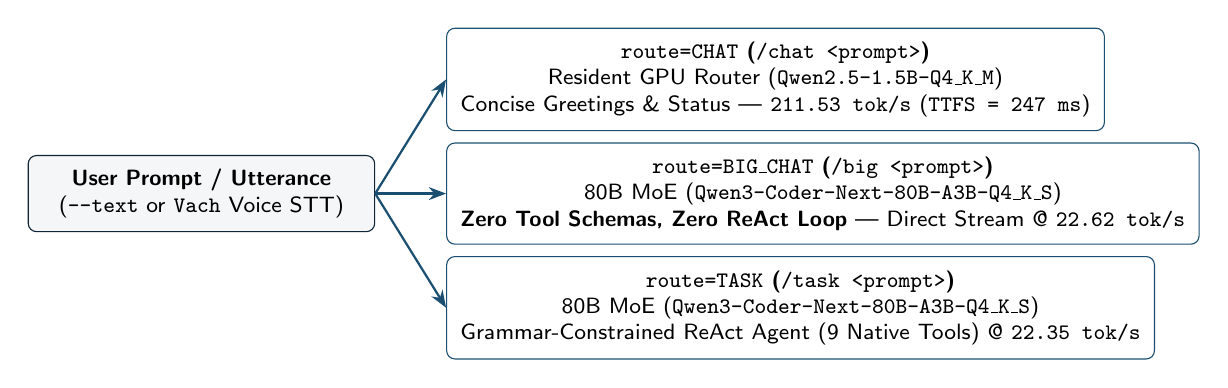
\begin{tikzpicture}[
  node distance=0.45cm and 0.7cm,
  box/.style={draw=arknavy, fill=arkgray, rounded corners=3pt, align=center, font=\sffamily\footnotesize, inner sep=5pt},
  route/.style={draw=arkblue, fill=white, rounded corners=3pt, align=center, font=\sffamily\footnotesize, minimum width=8.2cm, inner sep=5pt},
  arrow/.style={-{Stealth[length=2.2mm]}, thick, color=arkblue}
]
  \node[box, minimum width=4.4cm] (input) {\textbf{User Prompt / Utterance}\\(\texttt{--text} or \texttt{Vach} Voice STT)};
  \node[route, right=0.9cm of input, yshift=1.45cm] (chat) {\textbf{\texttt{route=CHAT} (\texttt{/chat <prompt>})}\\Resident GPU Router (\texttt{Qwen2.5-1.5B-Q4\_K\_M})\\Concise Greetings \& Status --- \textbf{\texttt{211.53 tok/s}} (\texttt{TTFS = 247 ms})};
  \node[route, right=0.9cm of input] (bigchat) {\textbf{\texttt{route=BIG\_CHAT} (\texttt{/big <prompt>})}\\80B MoE (\texttt{Qwen3-Coder-Next-80B-A3B-Q4\_K\_S})\\\textbf{Zero Tool Schemas, Zero ReAct Loop} --- Direct Stream @ \textbf{\texttt{22.62 tok/s}}};
  \node[route, right=0.9cm of input, yshift=-1.45cm] (task) {\textbf{\texttt{route=TASK} (\texttt{/task <prompt>})}\\80B MoE (\texttt{Qwen3-Coder-Next-80B-A3B-Q4\_K\_S})\\Grammar-Constrained ReAct Agent (9 Native Tools) @ \textbf{\texttt{22.35 tok/s}}};

  \draw[arrow] (input.east) -- (chat.west);
  \draw[arrow] (input.east) -- (bigchat.west);
  \draw[arrow] (input.east) -- (task.west);
\end{tikzpicture}
\end{center}

\subsection{Complete Feature Specification \& Rationale}
\begin{enumerate}[leftmargin=1.5em]
  \item \textbf{Why Separate \texttt{BIG\_CHAT} from \texttt{TASK}?} Coding-tuned 80B MoE models (\texttt{Qwen3-Coder-Next-80B-A3B}) presented with filesystem/shell tool schemas during a conceptual or mathematical query (e.g., \emph{``Explain Noether's Theorem''}) instinctively invoke \texttt{list\_dir} or \texttt{write\_file} instead of answering directly. \texttt{route=BIG\_CHAT} invokes the 80B MoE model with \textbf{zero tool schemas attached} and streams the full treatise directly to \texttt{stdout}, while \texttt{route=TASK} attaches the 9 native engineering tools (\texttt{read\_file}, \texttt{write\_file}, \texttt{list\_dir}, \texttt{make\_directory}, \texttt{run\_command}, \texttt{run\_readonly}, \texttt{read\_file\_system}, \texttt{ssh\_exec}, \texttt{ssh\_test}) inside a Yantra-supervised ReAct loop.
  \item \textbf{Zero Memory-Bleed Guard (\texttt{Sphinx/src/session.cpp}):} When \texttt{MemoryStore::retrieve} (backed by \texttt{Yantra::HnswIndex} across \texttt{Semantic}, \texttt{Episodic}, and \texttt{Correction} memories) returns zero relevant entries above the similarity threshold (\texttt{0.35f}), \texttt{Session::build\_system\_prompt} omits the memory section completely and instructs the assistant never to mention or apologize for missing persistent memory unless explicitly asked.
  \item \textbf{Real-Time Voice Vertical Slice:} Achieves \textbf{\texttt{149.53 ms}} conversational turn latency, \textbf{\texttt{0.024 ms}} barge-in cancellation, \textbf{\texttt{0.0000 ms}} inter-sentence audio gap across 3-sentence overlapped TTS synthesis, and \textbf{\texttt{20/20 (100\%)}} turn-router classification accuracy.
\end{enumerate}

% ============================================================================
% SECTION 13: LAYER 4.2 - MILDA
% ============================================================================
\section{Layer 4.2 --- \texttt{Milda} (\texttt{milda}): Polyglot 5-Language \& Esperanto C++23 Inference Engine}

\begin{itemize}[leftmargin=1.5em,itemsep=1pt]
  \item \textbf{Repository Path:} \texttt{\$HOME/AI/Arkantos/Milda} (and \texttt{/media/SphinxAI/Milda})
  \item \textbf{Public Headers:} \texttt{include/milda/engine.hpp}, \texttt{esperanto.hpp}, \texttt{hardware.hpp}, \texttt{milda\_i18n.hpp}
  \item \textbf{Installed Artifacts:} \texttt{build/milda} (CUDA Hybrid Workstation) \& \texttt{build-cpu/milda} (Portable Zero-CUDA CPU)
\end{itemize}

\subsection{Complete Feature Specification}
\begin{enumerate}[leftmargin=1.5em]
  \item \textbf{Five-Language Architecture (\texttt{eo}, \texttt{en}, \texttt{es}, \texttt{zh-Hans}, \texttt{ru}) \& Session Language Lock:}
  \begin{itemize}
    \item Locks the session language on the first user turn (\texttt{session\_lang\_locked\_}) and preserves it across all subsequent turns unless switched via \texttt{/lang} or an explicit natural-language request (\texttt{detect\_explicit\_language\_request}).
    \item \textbf{Token-Level Script Drift Guard (\texttt{is\_token\_violating\_language\_lock}):} Inspects sampled token candidates during decoding; if the locked language uses Latin script (\texttt{eo}, \texttt{en}, \texttt{es}) and a sampled token contains CJK ideographs (\texttt{U+4E00..U+9FFF}) or Cyrillic (\texttt{U+0400..U+04FF}), \texttt{Milda} suppresses the drifting token and selects the highest-probability valid-script token from the logit distribution.
  \end{itemize}
  \item \textbf{Zero-Allocation Esperanto \texttt{x}-System Transliteration \& REPL Commands:} In-place conversion of \texttt{cx}$\to$\texttt{\^c}, \texttt{gx}$\to$\texttt{\^g}, \texttt{hx}$\to$\texttt{\^h}, \texttt{jx}$\to$\texttt{\^j}, \texttt{sx}$\to$\texttt{\^s}, \texttt{ux}$\to$\texttt{\u{u}} and native Esperanto REPL controls (\texttt{/eliri}, \texttt{/vakigi}, \texttt{/konservi}, \texttt{/sxargi}, \texttt{/stat}, \texttt{/lang}, \texttt{/x-system}).
  \item \textbf{Gemma 4 \& Qwen3 Thought-Channel Suppression:} Pre-fills closed reasoning channels (\texttt{<|turn>model} \texttt{<|channel>thought<channel|>} on Gemma 4 and \texttt{<|im\_start|>assistant} \texttt{<think></think>} on Qwen3), filters any leaked thought blocks via a zero-allocation streaming state machine, and excises suppressed tokens from the KV cache after each turn.
  \item \textbf{Pinned System Prompt KV Checkpoint (\texttt{n\_keep\_}) \& Asymmetric Offloading:} Evaluates and pins the system prompt state (\texttt{pinned\_sys\_state\_}) once at startup for instant \texttt{/vakigi} resets, supports \texttt{--n-cpu-moe} and \texttt{--n-cpu-ffn} hybrid GPU+CPU execution across all 12 physical cores, and flushes \texttt{stdout} after every UTF-8 codepoint for zero-latency local and SSH streaming.
\end{enumerate}

% ============================================================================
% SECTION 14: LAYER 5 - STACK TEST
% ============================================================================
\section{Layer 5 --- \texttt{Stack Test} (\texttt{stack\_integration\_test}): Full-Stack Composability Proof}

Located at \texttt{\$HOME/AI/Arkantos/Stack Test/stack-integration}, \texttt{stack\_integration\_test} links exclusively against the installed packages in \texttt{\$HOME/.local} (\texttt{find\_package(Yantra REQUIRED)}, \texttt{find\_package(Sutra REQUIRED)}, \texttt{find\_package(Darshana QUIET)}) and verifies 7 hard composability seams against a live 7B GGUF model (\texttt{Qwen2.5-7B-Instruct-Q4\_K\_M.gguf}):

\begin{small}
\begin{tabularx}{\textwidth}{clY}
\toprule
\textbf{Check} & \textbf{Cross-Library Seam Verified} & \textbf{Hard Pass Criterion} \\
\midrule
\textbf{CHECK-1} & \texttt{Yantra::ModelRegistry} $\to$ \texttt{Sutra::LlamaCppClient} & Sutra loads the exact CAS path returned by Yantra; independent SHA-256 matches manifest SHA-256. \\
\textbf{CHECK-2} & \texttt{Sutra::AgentStats} $\to$ \texttt{Yantra::ExperimentStore} & 40 per-turn telemetry points (\texttt{ttft\_ms}, \texttt{total\_ms}, \texttt{tokens\_generated}, \texttt{tokens\_per\_sec}) across 10 live turns round-trip with $|\text{tracked} - \text{sutra}| < 10^{-6}$. \\
\textbf{CHECK-3} & \texttt{Sutra} Async Worker Pool $\to$ \texttt{Yantra::WalEngine} & All 10 turns log metrics concurrently from Sutra worker threads, producing 44 valid CRC32C WAL entries. \\
\textbf{CHECK-4} & \texttt{Yantra::RegistryError} $\to$ \texttt{Sutra::AgentError} & Missing-model \texttt{RegistryError} propagates through Sutra as a typed error (\texttt{is\_yantra\_registry\_error(err) == true}). \\
\textbf{CHECK-5} & \texttt{Yantra} Tracked Run $\to$ \texttt{Darshana::Spec} SVG & Darshana renders per-turn TTFT and total latency into valid vector \texttt{results-latency.svg}. \\
\textbf{CHECK-6} & End-to-End GGUF Artifact Integrity & Source GGUF SHA-256 equals Yantra CAS blob SHA-256. \\
\textbf{CHECK-7} & Full-Stack Teardown Memory Hygiene & Peak RSS $\le \text{model\_size} + 500\text{ MB}$; post-teardown RSS returns within $10\%$ of pre-run baseline. \\
\bottomrule
\end{tabularx}
\end{small}

% ============================================================================
% SECTION 15: GPLv3 + SECTION 7 EXCEPTION
% ============================================================================
\section{GPLv3 + Section 7 Runtime \& Hardware Compute Library Exception}

Every repository, source file, build script, and documentation manual in the \textbf{Arkantos AI Stack Suite} is distributed under the following license header:

\begin{lstlisting}
Copyright (C) 2026 Kival

This program is free software: you can redistribute it and/or modify
it under the terms of the GNU General Public License as published by
the Free Software Foundation, either version 3 of the License, or
(at your option) any later version.

Additional Permission under GNU GPL version 3 section 7 (Runtime &
Hardware Compute Library Exception):
As a special exception, the copyright holders of this program give you
permission to link or combine this program with NVIDIA CUDA Toolkit
libraries (including libcudart, libcublas, libcublasLt, libcurand,
libcufft, libcusparse, libcusolver, libnvrtc, and libcuda), Vulkan /
OpenGL / EGL / GLES drivers, SDL3, FreeType, HarfBuzz, ONNX Runtime,
espeak-ng, ALSA / PipeWire, llama.cpp / ggml, whisper.cpp, and standard
system/compiler runtime libraries, and to distribute the resulting
executable under terms of your choice, provided that the source code of
this program itself remains distributed under the terms of the GNU
General Public License version 3 or later.

This program is distributed in the hope that it will be useful,
but WITHOUT ANY WARRANTY; without even the implied warranty of
MERCHANTABILITY or FITNESS FOR A PARTICULAR PURPOSE.  See the
GNU General Public License for more details.

You should have received a copy of the GNU General Public License
along with this program.  If not, see <https://www.gnu.org/licenses/>.
\end{lstlisting}

% ============================================================================
% SECTION 16: FULL-STACK BUILD & MIRROR TOPOLOGY
% ============================================================================
\section{Full-Stack Dependency Build \& Synchronized Mirror Topology}

\subsection{Dependency-Order Build \& Verification Commands}
\begin{lstlisting}[language=bash]
export PREFIX="$HOME/.local"
export PKG_CONFIG_PATH="$PREFIX/lib/pkgconfig:$PKG_CONFIG_PATH"
export LD_LIBRARY_PATH="$PREFIX/lib:$LD_LIBRARY_PATH"

# 1. Hyper Math -> 2. Bellows -> 3. Basalt Deep Learning -> 4. ObsidianDb
cd "Hyper Math" && ./configure --prefix="$PREFIX" && make -j"$(nproc)" && make check && make install && cd ..
cd Bellows && make -j"$(nproc)" PREFIX="$PREFIX" HYPER_MATH_DIR="$(pwd)/../Hyper Math" && make check && make install PREFIX="$PREFIX" && cd ..
cd "Basalt Deep Learning" && ./configure --prefix="$PREFIX" && make -j"$(nproc)" && make check && make install && cd ..
cd Obsidian && ./configure --prefix="$PREFIX" && make -j"$(nproc)" && make check && make install && cd ..

# 5. Surya -> 6. Darshana -> 7. Yantra -> 8. Sutra -> 9. Vach -> 10. Sphinx -> 11. Milda
for comp in Surya Darshana; do
  cmake -S "$comp" -B "$comp/build" -DCMAKE_BUILD_TYPE=Release -DCMAKE_INSTALL_PREFIX="$PREFIX"
  cmake --build "$comp/build" -j"$(nproc)" && ctest --test-dir "$comp/build" --output-on-failure && cmake --install "$comp/build"
done
for comp in Yantra Sutra Vach; do
  cmake -S "$comp" -B "$comp/build-release" -DCMAKE_BUILD_TYPE=Release -DCMAKE_INSTALL_PREFIX="$PREFIX"
  cmake --build "$comp/build-release" -j"$(nproc)" && ctest --test-dir "$comp/build-release" --output-on-failure && cmake --install "$comp/build-release"
done
cmake -S Sphinx -B Sphinx/build/release -DCMAKE_BUILD_TYPE=Release -DCMAKE_INSTALL_PREFIX="$PREFIX"
cmake --build Sphinx/build/release -j"$(nproc)" && ctest --test-dir Sphinx/build/release --output-on-failure && cmake --install Sphinx/build/release
cmake -S Milda -B Milda/build -DCMAKE_BUILD_TYPE=Release -DMILDA_ENABLE_CUDA=ON
cmake --build Milda/build -j"$(nproc)" && ctest --test-dir Milda/build --output-on-failure
\end{lstlisting}

\subsection{Synchronized Workspace Roots \& Release Archives}
\begin{itemize}[leftmargin=1.5em,itemsep=2pt]
  \item \textbf{Primary Suite Workspace:} \nolinkurl{$HOME/AI/Arkantos}
  \item \textbf{Local Development Mirror:} \nolinkurl{$HOME/Coding/AI}
  \item \textbf{External Backup Suite Mirror:} \nolinkurl{/media/Backup/Coding/Antigravity/Artificial Intelligence}
  \item \textbf{Standalone Mirrors:} \nolinkurl{/media/Backup/Coding/Antigravity/{Basalt Deep Learning, Sphinx, Milda}} and \nolinkurl{/media/SphinxAI/Milda}
  \item \textbf{Source Release Archives (\texttt{Arkantos\_AI\_Stack\_Suite\_Source.zip}):}
  \begin{itemize}
    \item \nolinkurl{$HOME/Arkantos_AI_Stack_Suite_Source.zip}
    \item \nolinkurl{/media/SphinxAI/Arkantos_AI_Stack_Suite_Source.zip}
    \item \nolinkurl{/media/Backup/Coding/Antigravity/Arkantos_AI_Stack_Suite_Source.zip}
  \end{itemize}
\end{itemize}

\end{document}
